\documentclass[12pt]{article}

\usepackage[utf8]{inputenc}
\usepackage{graphicx}
\usepackage{fancyhdr}

\pagestyle{fancy}
\fancyhead[L]{Jeppe Møldrup}
\fancyhead[C]{Matematik 17}
\fancyhead[R]{09/04-2019}

\title{Matematik aflevering 17}
\author{Jeppe Møldrup}
\date{}

\begin{document}

\maketitle{}

\section*{Opgave 7}

I en model kan udviklingen beskrives ved
$$f(x) = b\cdot a^x$$
Hvor $f(x)$ betegner BNP pr. indbygger i USD til tidspunktet $x$ i år efter 1970.

a. Benyt tabellens data til at bestemme $a$ og $b$

Jeg laver eksponentiel regression på dataet og får

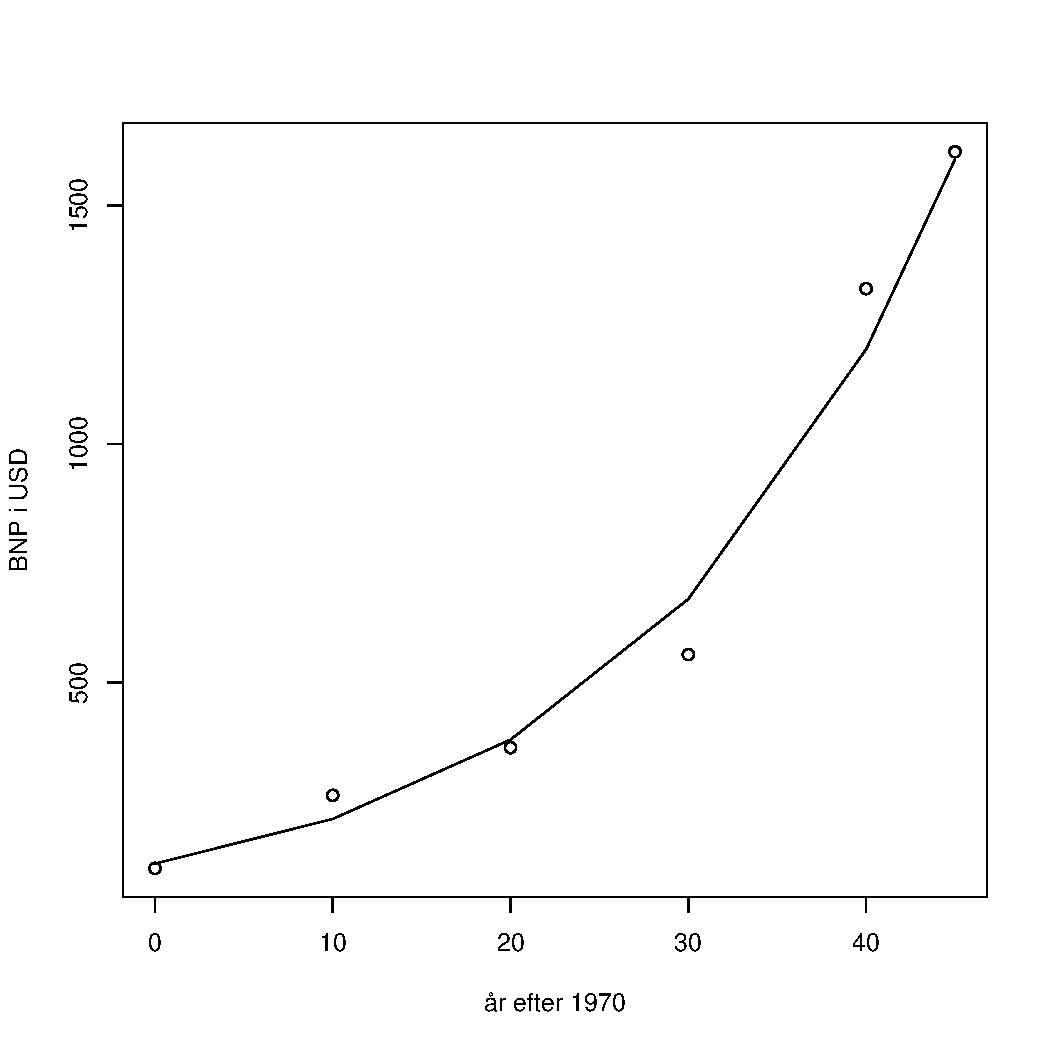
\includegraphics[width=\textwidth]{dia/7a.pdf}

a = 1.0570 og b = 120.847

b. Forklar betydningen af tallet $a$, og bestem fordoblingstiden

a er fremskrivningsfaktoren, som kan omregnes til raten med formlen
$$a = 1+r \Leftrightarrow r = 0.0570 = 5.7\%$$
Så raten er 5.7\%, dvs. BNP pr. indbygger øger med 5.7\% pr. år.

Fordoblingstiden findes med formlen
$$T_{1/2} = \frac{ln(2)}{ln(a)} = \frac{ln(2)}{ln(1.0570)} = 12.50$$
Så det tager 12.5 år før BNP pr. indbygger fordobles.

c. Benyt modellen til at bestemme det år, hvor BNP pr. indbygger overstiger 2000 USD.

Jeg indsætter 2000, og opstiller ligningen $2000 = 120.847\cdot(1.0570)^x$ og finder $x$ vha. solve
$$solve(2000 = 120.847\cdot(1.0570)^x,x) \rightarrow x = 50.6249$$
Så BNP pr. indbygger overstiger 2000 USD 50.6 år efter 1970, dvs. i år 2020

\section*{Opgave 8}

a. Bestem en ligning for den cirkel, der har centrum i $C$ og som går gennem punktet $P$.
$$C(5, 4)~~~~P(9, 3)$$
Cirklens ligning er givet ved
$$(x-x_0 )^2+(y-y_0 )^2 = r^2$$
Jeg finder $\vec{r}$ ved at finde vektoren fra centrum til punktet på cirklen
$$\vec{r} = \vec{CP} = \begin{pmatrix} 9-5 \\ 3-4 \end{pmatrix} = \begin{pmatrix} 4 \\ -1 \end{pmatrix}$$
Længden af vektor r er
$$r = |\vec{r}| = \sqrt{4^2+(-1)^2} = \sqrt{17}$$
$$r^2 = 17$$
Så indsætter jeg i cirklens ligning som bliver
$$C:~~(x-5)^2+(y-4)^2=17$$

b. Bestem en ligning for tangenten $t$ til cirklen i punktet $P$

En tangent til en cirkel vil have normalvektoren der går fra cirklens centrum til røringspunktet, i dette tilfælde betyder det at
$$\vec{n} = \vec{r} = \begin{pmatrix} 4 \\ -1 \end{pmatrix}$$
Og linjens ligning er givet ved
$$a(x-x_0)+b(y-y_0) = 0$$
Så jeg indsætter
$$4(x-9)-1(y-3) = 0 \Leftrightarrow y=4x-33$$
Så tangentens ligning er $y=4x-33$

c. Bestem koordinatsættet til denne tangents røringspunkt med cirklen.

Jeg ved at da det er en cirkel, og at den anden tangent er parallel med den første, skal rørtingspunkterne ligger i hver
sin side af cirklen, idet der er 180 grader mellem de to punkter. Så for at finde det andet røringspunkt. skal jeg finde
$$\vec{OP_2} = \vec{OC}-\vec{r} = \begin{pmatrix} 5-4 \\ 4+1 \end{pmatrix} = \begin{pmatrix} 1 \\ 5 \end{pmatrix}$$
Så det andet røringspunkt er $P_2(1, 5)$

\section*{Opgave 9}

a. Benyt modellen til at bestemme størsteværdi og mindsteværdi for døgnets middelntemperatur.

$$T(x) = 15\cdot sin(0.0172x-1.5)+8$$
Idet det eneste i funktionen der varierer er sinus, og den maksimale værdi sinus kan antage er 1 og den mindste er -1, kan jeg bare
indsætte de to værdier ind i funktionen for at finde minimum og maksimum som er
$$T_{maks} = 15\cdot 1+8 = 23$$
$$T_{min} = 15\cdot (-1)+8 = -7$$
Så minimummiddeltemperaturen er -7 og maksimummiddeltemperaturen er 23

\section*{Opgave 10}

a. Opstil en nulhypotese, der kan benyttes til at undersøge, om læsehastigheden efter læseforløbet er uændret, og bestem de tilhørende forventede værdier.

Jeg opstiller nulhypotesen, H0: Eleverne har på et 5 procents signifikansniveau ikke forbedret sig. For at udregne de forventede værdier, ganger
jeg den forventede procentdel med det totale antal af elever, f.eks. for elever ved 80-110 ord/minut
$$0.31\cdot 150 = 46.5$$
Så den forventede værdi hvis der ingen forbedring er i gruppen 80-110 ord/minut er 46 elever. Alle forventede værdier er så
\begin{center}
\begin{tabular}{c c c c c}
        13.8 & 46.5 & 61.95 & 22.65 & 5.1 \\
\end{tabular}
\end{center}

b. Benyt et statistisk test med et signifikansniveau på 5\% til at afgøre, om nulhypotesen kan forkastes

Jeg laver en $\chi ^2$-GOF test på dataet og får resultaterne
$$\chi ^2 = 12.1509 ~~~~ P-value = 0.0163$$
Så idet $P<0.05$ bliver vi nødt til på 5\% signifikansniveau at forkaste nulhypotesen og acceptere, at børnene er blevet bedre til at læse

\section*{Opgave 11}

a. Benyt modellen til at bestemme det årlige antal fødsler i Danmark i år 2020

$$N(t) = \frac{20414}{1+6.325\cdot e^{-0.378\cdot t}}+54349$$
t er målt i år efter 2014, så jeg indsætter 6 på t's plads
$$N(6) = 66685.55 \approx 66685$$
Så i år 2020 er der ifølge modellen cirka 66685 fødsler.

b. Bestem $N'(4)$, og giv en fortolkning af dette tal

Jeg differentierer og indsætter 4
$$\frac{d}{d4}(N(4)) = 1876$$
Dette er den årlige ændring i fødsler i år 2018, dvs. at i år 2018, kommer der 1876 ekstra fødsler til pr. år.

\section*{Opgave 12}

a. Bestem arealet af $M$

$$f(x) = -x^2+4x$$
Jeg starter med at finde rødderne, dvs. der hvor $f(x) = 0$ vha. solve
$$solve(-x^2-4x = 0, x) \rightarrow x=0 \vee x=4$$
Så integrerer jeg mellem de to rødder for at finde arealet under grafen ned til 1. aksen.
$$M = \int_0^4 f(x) dx = 10.67$$
Så arealet af $M$ er 10.67

b. Bestem $K$, så arealerne af $M_1$ og $M_2$ er lige store.

$$g(x) = k\cdot x,~~~~0<k<4$$
Jeg starter med at finde en funktion for skæringspunkterne, ved at substituerer de to funktioner idet de vil have samme koordinater i skæringspunkterne
$$-x^2+4x=k\cdot x$$
Idet $x$ indgår i alle led ved vi at punktet $x = 0$ er en løsning. Så kan jeg dividerer med $x$ som eleminerer løsningen $x = 0$
og derfor giver en funktion for det andet skæringspunkt
$$-x+4 = k \Leftrightarrow x = -k+4$$
Så kan jeg finde punktet ved at finde hvilken værdi af $k$ det ene areal er lig med halvdelen af 10.67. Idet
arealet bliver skåret i to dele, ved jeg at den anden del så vil være det resterende, og dermed også halvdelen af 10.67.
Dette gør jeg vha. solve
$$solve \left( \int_0^{-k+4} f(x) dx-\int_0^{-k+4} k\cdot x dx = \frac{10.67}{2},k \right) \rightarrow k = 0.83$$

Så hvis arealet $M$ skal deles af $g(x)$ i to lige store dele, skal $k$ have værdien 0.83.

\section*{Opgave 13}

a. Bestem koordinatsættet til hvert af skæringspunkterne.

$$K:~~(x-3)^2+(y+4)^2+(z-2)^2=9$$
$$\alpha:~~2x-2y+z-30=0$$

Normalvektoren fra $\alpha$ er retningsvektor for linjen $l$. Jeg aflæser den ud fra $\alpha$ til at være
$$\vec{n_\alpha} = \vec{r} = \begin{pmatrix} 2 \\ -2 \\ 1 \end{pmatrix}$$
Ud fra kuglens ligning, aflæser jeg at kuglens radius er $\sqrt{9} = 3$. Længden af retningsvektoren er $\sqrt{2^2+(-2)^2+1^2} = \sqrt{9} = 3$. Da
retningsvektoren er ligeså lang som radius af kuglen. Kan jeg finde skæringspunkterne ved $p = \vec{Oc} \pm \vec{r}$ hvor c er kuglens centrum.
Idet retningsvektoren er parallel med linjen
$$\vec{Oc} + \vec{r} = \begin{pmatrix} 3+2 \\ -4-2 \\ 2+1 \end{pmatrix} = \begin{pmatrix} 5 \\ -6 \\ 3 \end{pmatrix}$$
$$\vec{Oc} - \vec{r} = \begin{pmatrix} 3-2 \\ -4+2 \\ 2-1 \end{pmatrix} = \begin{pmatrix} 1 \\ -2 \\ 1 \end{pmatrix}$$
Så de to skæringspunkter er
$$P_1(5, -6, 3)~~~~~P_2(1, -2, 1)$$

b. Bestem afstanden fra $\alpha$ til det punkt på kuglen $K$, der er tættest på $\alpha$.

Idet skæringspunkterne fra a ligger på den rette linje mellem kuglens centrum og planen, er et af dem den der ligger tættest på planen.
Afstanden mellem et punkt og en plan er givet ved formlen
$$dist(\alpha, P) = \frac{|ax_1+by_1+cz_1+d|}{\sqrt{a^2+b^2+c^2}}$$
Så jeg indsætter de to punkter
$$dist(\alpha, P_1) = \frac{|2\cdot 5+(-2)\cdot (-6)+1\cdot 3+(-30)|}{\sqrt{2^2+(-2)^2+1^2}} = 1. \overline{6}$$
$$dist(\alpha, P_2) = \frac{|2\cdot 1+(-2)\cdot (-2)+1\cdot 1+(-30)|}{\sqrt{2^2+(-2)^2+1^2}} = 7. \overline{6}$$
Så det punkt der ligger tættest på er $P_1$ som ligger $1. \overline{6}$ fra planen.

\section*{Opgave 14}

a. Bestem en forskrift for $f$.

Koppen har i bunden radius på 3, dvs. skæringspunktet med y-aksen for $f$ skal være (0, 3). Derudover
har den ved 11 cm højde, en radius på 5, så derfor ved jeg at $f$ skal skære punktet i (11, 5).
For en linæer sammenhæng gælder det at
$$a = \frac{y_2-y_1}{x_2-x_1} = \frac{5-3}{11-0} = \frac{2}{11}$$
$b$ betegner skæringen med $y$, som vi kender fra det første punkt. Så derfor har $f$ forskriften
$$f(x) = \frac{11}{2}x+3$$

b. Benyt modellen til at bestemme volumenet af kaffe i bægeret.

Der bliver hældt kaffe fra 0 cm op til 8 cm. For at finde volumenet finder jeg omdrejningslegemet af funktionen
$f(x)$ i området fra 0 til 8 med formlen
$$v = \int_a^b (f(x))^2 dx$$
Så jeg indsætter
$$v = \int_0^8 (\frac{2}{11}x+3)^2 dx = 353.6\ cm^3 = 353 mL$$
Så volumenet af kaffen er 353 mL

\section*{Opgave 15}

a. Bestem en forskrift for $C(t)$, og tegn grafen for $C$.

$$C' = 2\cdot t\cdot \frac{30-C}{30},~~~~0<=t<=10$$
$$C(0) = 0$$
For at finde forskriften for $C(t)$ benytter jeg desolve
$$desolve \left( C'=2\cdot t\cdot \frac{30-C}{30}~and~C(0)=0,t,C \right) \rightarrow C(t) = 30-30e^{-t^2\cdot 30^-1}$$
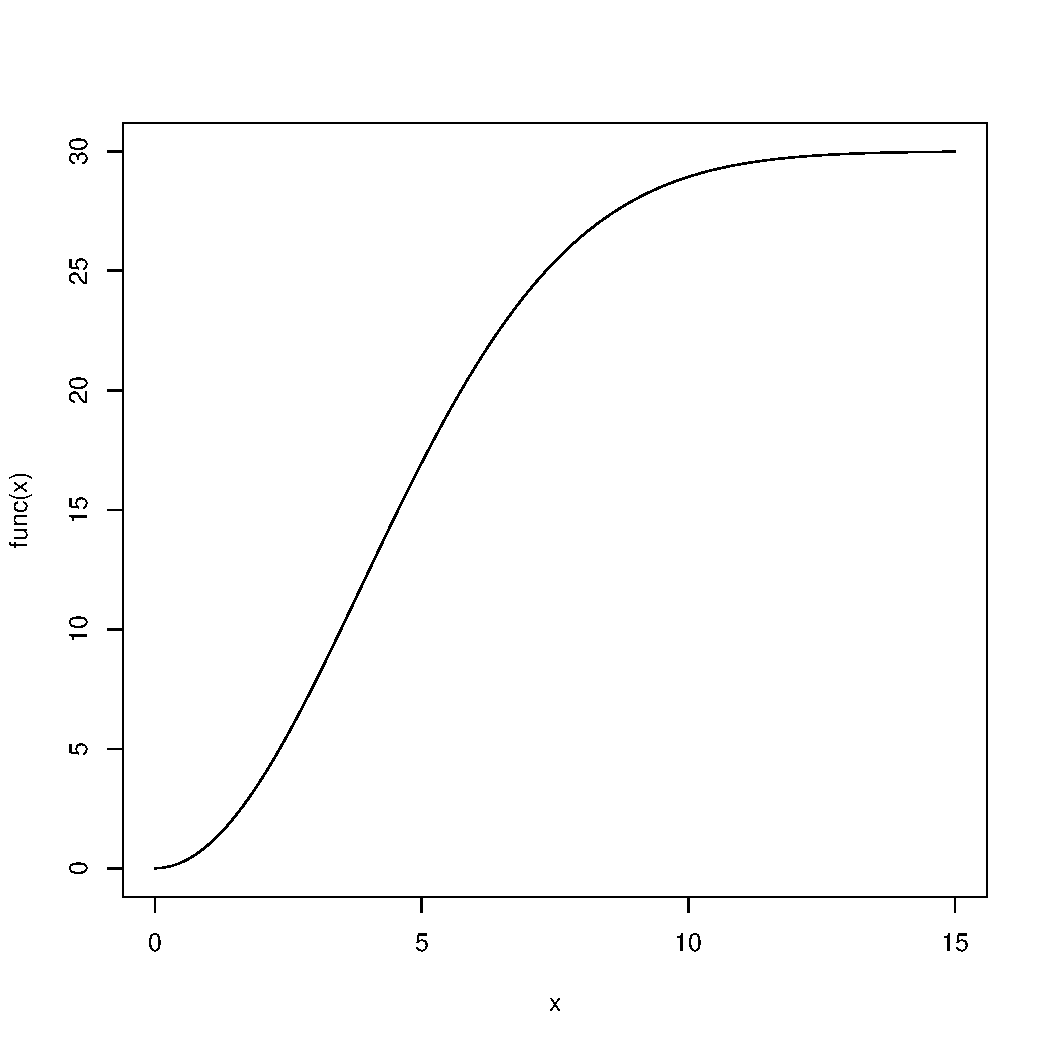
\includegraphics[width=\textwidth]{dia/15a.pdf}
Forskriften er altså
$$C(t) = 30-30e^{-t^2\cdot 30^-1}$$

b. Bestem det tidspunkt, hvor koncentrationen af stoffet i beholderen vokser hurtigst.

Idet jeg skal finde den hurtigste ændring, er det det højeste punkt i den afledte jeg skal finde.
Så derfor finder jeg alle mulige ekstremaer i den afledte, dvs. punkter hvor $C''(t) = 0$ vha. solve
$$C'' = \frac{d^2}{dt^2}(C(t)) = (2-\frac{2t^2}{15})e^{-t^2\cdot 30^-1}$$
$$solve(C''(t) = 0, t) \rightarrow t = \sqrt{15}$$
Så kigger jeg på området før og efter punktet for at finde ud af om det er et maksimum, minimum eller en vandret vendetangent.
$$C''(\sqrt{14}) = 0.08~~~~C''(4) = -0.07$$
Idet grafen stiger før, og aftager efter ved jeg at punktet i $t = \sqrt{15}$ er det punkt hvor koncentrationen af stoffet i beholderen vokser hurtigst

\end{document}
